\begin{enumerate}
    \item A thin convex lens is made of two materials with refractive indices \(n_1\) and \(n_2\), as shown in figure. The radius of 
curvature of the left and right spherical surfaces are equal. \(f\) is the focal length of the lens when \(n_1 = n_2 = n\). The focal length
is \(f + \Delta f\) when \(n_1 = n\) and \(n_2 = n + \Delta n\). Assuming \(\Delta n \ll (n - 1)\) and \(1 < n < 2\), the correct 
statement(s) is/are,
        \begin{tasks}(2)
            \task \(|\frac{\Delta f}{f}| < |\frac{\Delta n}{n}|\)
            \task For \(n = 1.5\), \(\Delta n = 10^{-3}\) and \(f = 20\) cm, the value of \(|\Delta f|\) will be 0.02 cm (round off to 
2\(^{nd}\) decimal place).
            \task If \(\frac{\Delta n}{n} < 0\) then \(\frac{\Delta f}{f} > 0\)
            \task The relation between \(\frac{\Delta f}{f}\) and \(\frac{\Delta n}{n}\) remains unchanged if both the convex surfaces are 
replaced by concave surfaces of the same radius of curvature.
        \end{tasks}
    \begin{center}
        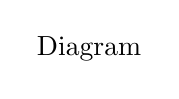
\begin{tikzpicture}
            \node {Diagram};
        \end{tikzpicture}
    \end{center}
\end{enumerate}